\chapter{Диаграммы классов}
    После определения технологий программирования был начат этап %
    разработки диаграммы классов. В процессе исследования хороших %
    практик разработки веб-приложений было принято решение использовать %
    паттерн проектирования “Модель-Представление-Контроллер”. Данный %
    паттерн был выбран, потому что он позволяет логически разделить %
    функции приложения на компоненты, что упрощает работу с проектом. %
    Кроме того, данный паттерн позволяет создать динамичный веб-сайт, %
    это является преимуществом, так как данный проект должен адаптироваться %
    под пользователя.

    В выбранной библиотеки для разработки приложения данный паттерн %
    проектирования реализуется при помощи следующих базовых классов:
    \begin{itemize}
        \item Моделью в библиотеке “Django” представляется класс “Model”. %
        Как правило, модель наследуется от данного базового класса и содержит %
        атрибуты, представляющие поля базы данных, а также методы для работы и %
        обработки информации, которые содержаться в атрибутах класса.
        \item Контроллером в библиотеке представляется класс “Serializer”, %
        в частности класс “ModelSerialzier”. Данный класс позволяет интерпретировать %
        действия пользователя оповещая модель о необходимости изменения.
        \item Представлением является класс “APIVIew”. %
        Данный класс позволяет обрабатывать HTTP запросы и возвращать %
        ответ в формате JSON при помощи сериализаторов, которые выступают в роли  контроллера. 
    \end{itemize}

    \section{Составление диаграммы классов моделей}
        Использование библиотеки “Django” \cite{django} для %
        разработки веб-приложения позволяет использовать предоставленный %
        базовый класс модели, который реализует механизм  объектно-реляционного %
        отображение (ORM) классов. В соответсвии с разработанной схемой базы данных %
        были спроектированы классы-модели. Диаграмма классов предоставлена %
        на рисунке \ref{class-diagram-models}.

        \begin{landscape}
            \begin{figure}[H]%current location
                \centering
                \scalebox{0.5}{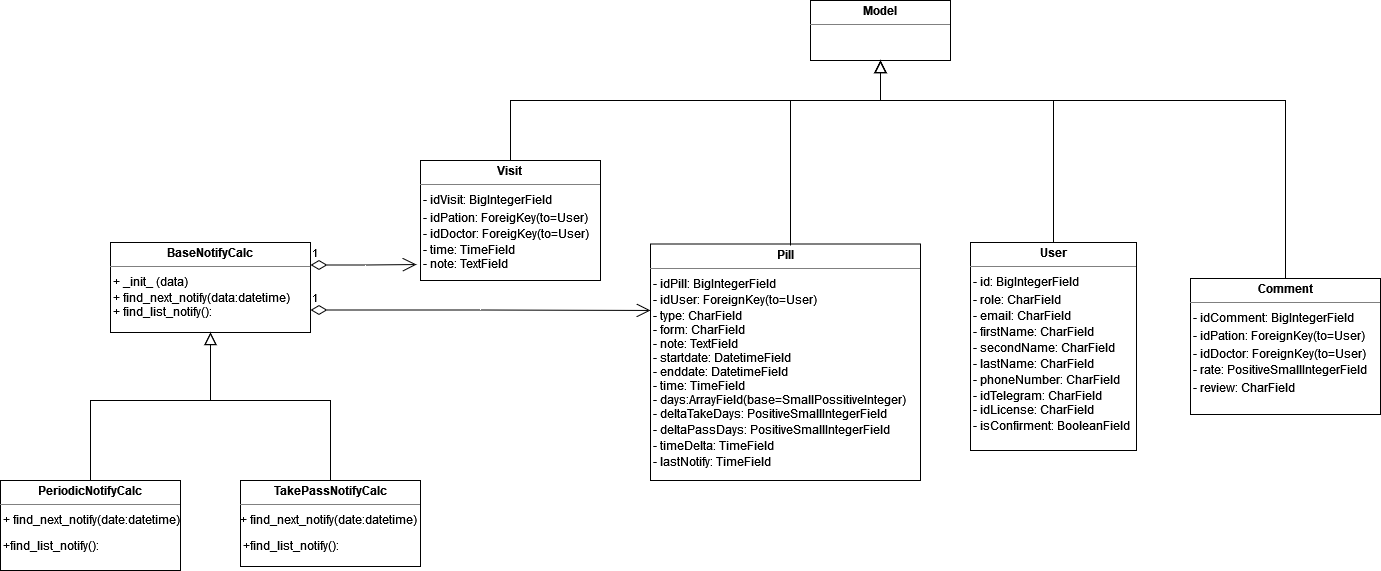
\includegraphics{pics/class-diarams/models.png}}
                \caption{Диаграмма классов моделей.} \label{class-diagram-models}
            \end{figure} 
        \end{landscape}

        Каждый представленный на диаграмме \ref{class-diagram-models}  отображает таблицу в %
        базе данных. От класса “Model” наследуются “Pill”, “Visit”, “User”, “Comment”. %
        Данное наследование обоснованно необходимостью использования механизма объектно-реляционного %
        отображения. Также, каждый атрибут перечисленных классов является классом, %
        который предоставляется в библиотеке “Django” \cite{django}, для корректного %
        преобразования информации из базы данных.

        Для реализации логики нахождения времени уведомления в класс “Pill”, который %
        отображает сущность “Прием препаратов”, был добавлен атрибут “data\_calc”. %
        Данный атрибут является классом-фабрикой. Данный класс возвращает необходимый %
        класс калькулятора для нахождения времени уведомления для пользователя на %
        основании типа приема. Класс “BaseNotifyCalc” содержит в себе методы %
        “find\_next\_notify” и “find\_list\_notify”. Эти методы возвращают следующую дату %
        уведомления и список дат, когда должно прийти уведомление о приёме лекарства. В %
        следствии эти методы будут перегружены в классах наследниках “PeriodNotifyCalc” и %
        “TakePassNotifyCalc”. В родительском классе происходит расчет дат уведомлений, исходя %
        из того, что пациент принимает лекарство каждый день в определённое время. В классах %
        “PeriodNotifyCalc” и “TakePassNotifyCalc” - пациент принимает лекарство через %
        фиксированное количество дней в определённое время, или пациент принимает лекарство %
        подряд несколько дней и делает паузу на определённое количество дней соответственно. 
        
    \section{Составление диаграммы классов контроллеров}
        Благодаря библиотеке “Django” были спроектированы классы выполняющие %
        функцию сериализации при помощи наследования от класса “ModelSerialiser”, %
        который предоставляет возможность создать контроллеры, работающие с экземплярами %
        моделей и наборами запросов.

        В соответствии с разработанными классами-моделями были созданы %
        классы для сериализации. Диаграмма классов изображена на рисунке \ref{class-diagram-serializers}.
        \begin{landscape}
            \begin{figure}[H]%current location
                \centering
                \scalebox{0.55}{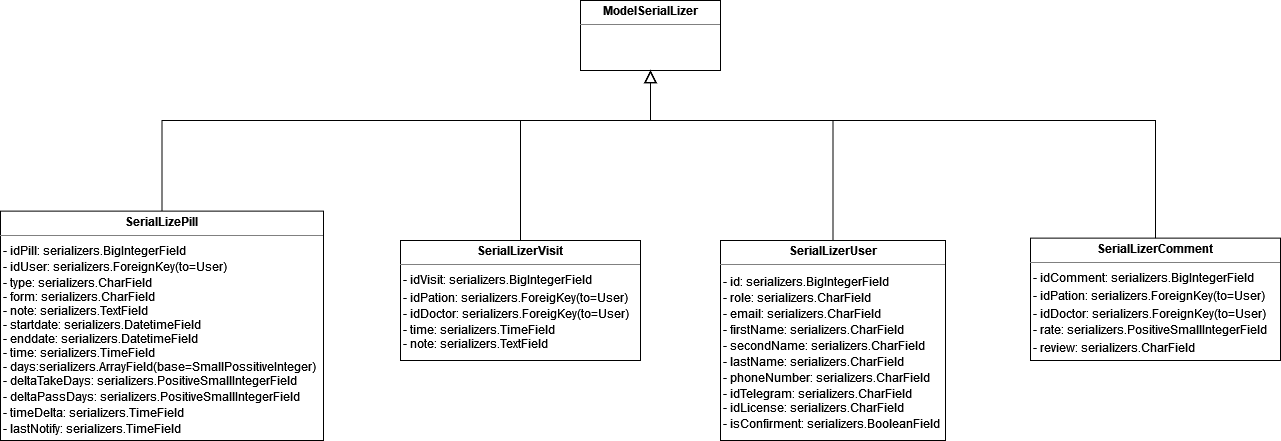
\includegraphics{pics/class-diarams/serializers.png}}
                \caption{Диаграмма классов контроллеров.} \label{class-diagram-serializers}
            \end{figure} 
        \end{landscape}

        Классы сериализаторов “SerialLizePill”, “SerialLizerUser”, %
        “SerialLizerVisit”, “SerialLizerComment” созданы для сериализации %
        данных классов “Pill”, “User”, “Visit”, “Comment” в JSON или XML. %
        Так же стоит заметить, что для всех атрибутов используется Field %
        класса “Serializer” для представления отношений, в которых один тип %
        объекта вложен в другой. Для указанных вложенных представлений будут %
        указаны флаги “required=False” и “many=True” в случае, если вложенное %
        представление может опционально принимать значение None или если вложенное %
        представление должно быть списком элементов соответственно.

    \section{Составление диаграммы классов представлений}
        Функцию представлений в используемой библиотеке выполняет класс ViewSet, %
        который позволяет обрабатывать все запросы, связанные с операциями удаления, %
        получения, изменения и обновления модели при помощи контроллера. Данный класс %
        реализуется при помощи наследования от базового класса “ViewsSet” и указанием %
        используемого контроллера для взаимодействия и интерпретирования пользовательских %
        действий, который изменяют состояние используемой модели. Диаграмма классов %
        изображена на рисунке \ref{class-diagram-views}.

        \begin{figure}[H]%current location
            \centering
            \scalebox{0.5}{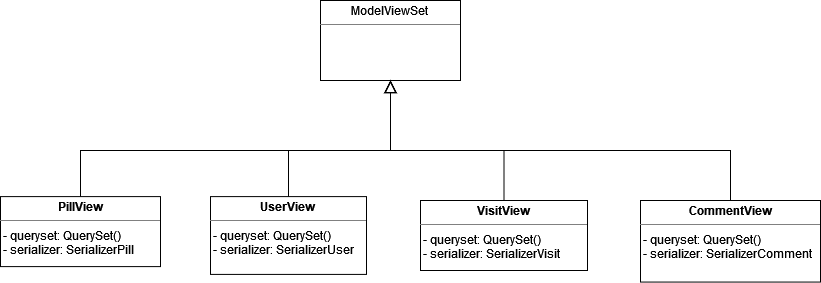
\includegraphics{pics/class-diarams/views.png}}
            \caption{Диаграмма классов представлений.} \label{class-diagram-views}
        \end{figure} 
    
    \section{Составление диаграммы классов сериализации и представлений}
        В указанных выше пунктах были созданы классы представлений и сериализации. %
        В результате была создана итоговая диаграмма. Диаграмма классов изображена на рисунке %
        \ref{class-diagram-views-serializer}.

        \begin{landscape}
            \begin{figure}[H]%current location
                \centering
                \scalebox{0.42}{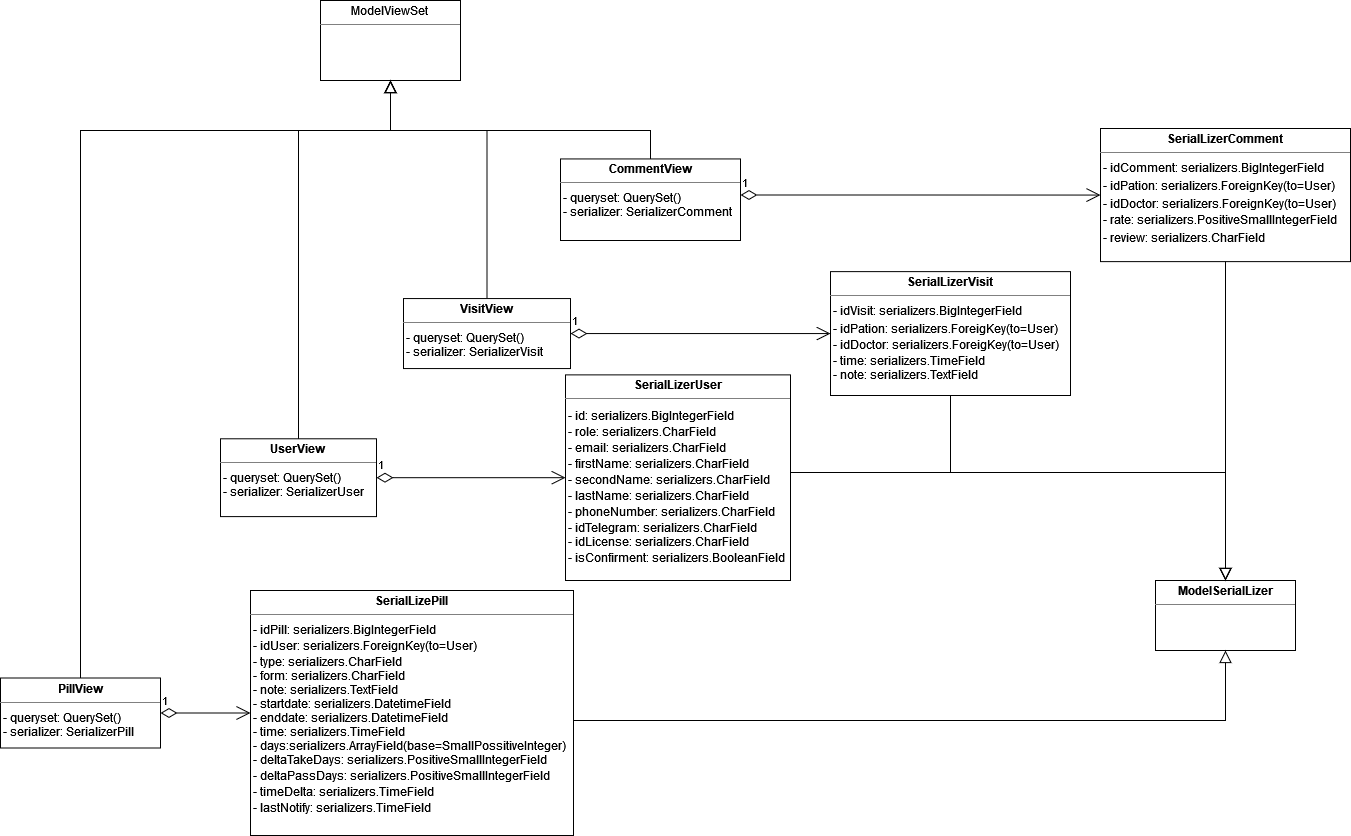
\includegraphics{pics/class-diarams/views-serializers.png}}
                \caption{Общая диаграмма классов.} \label{class-diagram-views-serializer}
            \end{figure}
        \end{landscape}
        
        На данной диаграмме можно заметить, что между соответствующими классами %
        представления и классами сериализаторов реализована агрегация. Это необходимо, %
        потому что это неотъемлемая часть представления, показывающая какой класс %
        сериализатора использовать. 

        Таким образом была создана иерархия классов для данного проекта. Основываясь на %
        ней в будущем будет возможность удобно добавлять новые функции по %
        мере роста проекта. Также на данном этапе иерархия поможет непосредственно в %
        создании проекта и в реализации общения с базой данных.